% --------------------------------------------------------------------------
% Template for WASPAA-2019 paper; to be used with:
%          waspaa17.sty  - WASPAA 2019 LaTeX style file, and
%          IEEEbib.bst - IEEE bibliography style file.
%
% --------------------------------------------------------------------------

\documentclass{article}
\usepackage{waspaa17,amsmath,amssymb,graphicx,url,times}
\usepackage{color}
\usepackage{tabularx,booktabs,colortbl}
\usepackage{hyperref,subfig}
% Example definitions.
% --------------------
\def\defeqn{\stackrel{\triangle}{=}}
\newcommand{\symvec}[1]{{\mbox{\boldmath $#1$}}}
\newcommand{\symmat}[1]{{\mbox{\boldmath $#1$}}}
\raggedbottom
% Title.
% --------------------
% \title{Estimation of Guitar String, fret and plucking position using a physical model and no training data}
\title{ Improved physical models for fast estimation of guitar string, fret and plucking position}
%\title{Estimation of Guitar String, fret and plucking position using a simulation of the inharmonic string}
% ---------------
\name{Jacob~M\o ller Hjerrild, Silvin Willemsen and~Mads~Gr\ae sb\o ll~Christensen}%\thanks{Thanks to XYZ agency for funding.}}
\address{Audio Analysis Lab, CREATE, Aalborg University, Denmark\\
   \texttt{\{jmhh, sil, mgc\}@create.aau.dk}}
%
\begin{document}
\ninept
\maketitle
\begin{sloppy}
%%%%%%%%%%%%%%%%%%%%%%%%%%%%%%%%%%%%%%%%%%%%%%%%%%%%%
%%%%%%%%%%%%%%%%%%%% ABSTRACT %%%%%%%%%%%%%%%%%%%%%%%
%%%%%%%%%%%%%%%%%%%%%%%%%%%%%%%%%%%%%%%%%%%%%%%%%%%%%
\begin{abstract}
  In this paper a method for analyzing guitar performances is proposed. This method extracts the activated string and fret as well as the plucking position, and it is purely based on a physical model of string excitation and vibration, hence it does not require any training data which makes it fast and effective. Since it operates on a 40 ms segment-by-segment basis it is suitable for real-time estimation...
\end{abstract}
%
\begin{keywords}
 Physical Modeling, Statistical Signal Processing, Parametric Pitch Estimation, Music Information Retrieval\vspace{-.8mm}
 \end{keywords}
%
%%%%%%%%%%%%%%%%%%%%%%%%%%%%%%%%%%%%%%%%%%%%%%%%%%%%%
%%%%%%%%%%%%%%%%%%%% INTRODUCTION %%%%%%%%%%%%%%%%%%%
%%%%%%%%%%%%%%%%%%%%%%%%%%%%%%%%%%%%%%%%%%%%%%%%%%%%%
\section{Introduction}
\label{sec:intro}
The analysis of individual instruments in musical performances has various applications, such as music learning, detailed transcription, artist recognition and extraction of stylistic details. Analysis and synthesis of plucked string instruments have been studied for electric~\cite{sullivan1990extending} and acoustic guitars~\cite{Karjalainen93towardshigh-quality,laurson2001methods}. The present study is concerned with the analysis of guitar string signals and we present a detailed transcription here. To date, there are few papers on extracting information from electric guitar signals, such as the work concerned with classifying the types of effects used~\cite{abesser2012feature} and estimating decay times of electric guitar tones~\cite{pate2014predicting}. Other research involved the extraction of information from plucked string instruments, such as extracting plucking styles and dynamics for classical guitar~\cite{erkut2000extraction} and electric bass guitar~\cite{abesser:automatic_string_detection_ml}. Recent papers introduce models of the physical interactions between player and string to make synthesized guitar sound more realistic, such as the modeling of interactions with the string and guitar pick~\cite{germain2009synthesis,evangelista2010player} or the fingers~\cite{poirot_nonlinear_interactions_with_string}, and the fingers with the fretboard~\cite{bilbao2015numerical}. 

It is well-known that the transducer position and plucking position produce a comb-filtering effect in the guitar signal spectrum~\cite{fletcher:physics_of_musical_instruments} and that stringed instruments are inharmonic because of stiffness in the string~\cite{fletcher:principles_of_vibration_and_sound}. Inharmonicity is also related to the plucking deflection as shown in~\cite{donkin:acoustics,rayleigh:sound,coltShank,rossing:science_of_string_instruments}. The inharmonicity has been proven useful for detailed transcription~\cite{barbancho:inharmonicity_tablature}, which is a topic that is only beginning to emerge, wherein not only notes are identified but also where and how they were played (i.e. string, fret and plucking positions). As shown in~\cite{dittmar:realtime_string_detection}, a string and fret classification method was proposed using a 10-dimensional feature set and a SVM classifier. In~\cite{abesser:automatic_string_detection_ml}, the electric guitar strings were distuingished with a string model comprising a 48-dimensional feature set~\cite{abesser:automatic_string_detection_ml}, wherein the inharmonicity coefficient was selected as one of the most discriminative features. Large feature sets are prone to overfitting and rarely contribute to meaningful cause and effect findings and complex algorithms can have a high computational cost. 
To overcome such problems, Barbancho et al.~\cite{barbancho:inharmonicity_tablature} proposed an inharmonicity and amplitude based method for accurate generation of guitar tablature; assuming a known fundamental frequency, and the main parameter for classification of string and fret was based on counting the number of partials that follow the piano model which was derived in~\cite{fletcher:piano_model}. Recently, Michelson et al.~\cite{michelson2018_aes} extended on~\cite{barbancho:inharmonicity_tablature} and proposed to classify string and fret by modeling each inharmonicity coefficient as a Gaussian distribution. Both methods~\cite{barbancho:inharmonicity_tablature,michelson2018_aes} operate on multiple segments, each in the order of 100 ms, which makes them unsuitable for high-tempo and real-time applications. To overcome such problems~\cite{hjerrild::icassp19} proposed a fast inharmonic parametric pitch estimation algorithm that operates on a single 40 ms segment to estimate string, fret and the plucking position. The methods presented in~\cite{barbancho:inharmonicity_tablature,michelson2018_aes,hjerrild::icassp19} require training data in the form of audio recordings to build a model of the guitar, which can be very many, i.e., for 6 strings and 12 frets that is $K=72$  classes. Although~\cite{hjerrild::icassp19,barbancho:inharmonicity_tablature} shows that a model can be trained from audio recordings captured from only one fret per string, there are three main challenges associated with such a a fast training procedure, i.e.,
\begin{itemize}
    \item With only a few observations (i.e. 10 per string~\cite{hjerrild::icassp19}), it is impossible to conclude anything significant on the covariance structure of each class in the feature space.
    \item Although training is relatively fast, it is required for every different set of guitar strings.
        \item There is no information of class dependent distributions in the observed feature space, i.e. covariance structures. Except from the 6 classes represented in the training set.
\end{itemize}
In this paper, we extend the work of~\cite{hjerrild::icassp19} by eliminating the training procedure that requires the user to provide recordings and as we shall see, we obtain detailed and class dependent distributions in the feature space. Instead of training a model from audio recordings, we propose to simulate a model of guitar string vibrations based on physical properties of the string, given from string dimensions and materials including a generalized model of the plucking force. Detailed information of string properties are often available on string packets and in datasheets. The objective of the propoied meshodt s to extract the location of interactions of both hands of the guitar player when these can be arbitrarily located along a string. This is done on a segment-by-segment basis and requires no audio retordingscf r oraining, but information about string properties, such that the proposed method is suitable for high-tempo and real-time applications. The feature set is extracted with the parametric pitch estimation method of~\cite{hjerrild::icassp19} and consists of fundamental frequency $\omega_0$ and inharmonicity $B$, which we model in detatl in ihe proposed simulation. Figure~\ref{fig:guitar_overview} gives an overview of the guitar, where the right hand controls plucking position and the left hand controls pitch by using the fretboard. One pitch is produced in various positions and each string and fret combination is defined as one class, such that we have a set of $K$ mutually exclusive classes. 
%
%%%%%%%%%%%%%%%%%%%%%%%%%%%%%%%%%%%%%%%%%%%%%%%%%%%%%
%%%%%%%%%%%%%%%%%%%% SIGNAL MODEL %%%%%%%%%%%%%%%%%%%
%%%%%%%%%%%%%%%%%%%%%%%%%%%%%%%%%%%%%%%%%%%%%%%%%%%%%
%
\newcommand{\ts}{\textsuperscript}

\newcommand{\fret}{f}


\newcommand{\veca}{\mathbf a}
\newcommand{\vecx}{\mathbf x}
\newcommand{\vecs}{\mathbf s}
\newcommand{\vecv}{\mathbf v}
\newcommand{\matV}{\mathbf V}
\newcommand{\vecz}{\mathbf z}
\newcommand{\vecX}{\mathbf X}
\newcommand{\mtrxsigma}{\mathbf{\Sigma}}
\newcommand{\argmax}[1]{\underset{#1}{\operatorname{argmax}}\;}
\newcommand{\argmin}[1]{\underset{#1}{\operatorname{argmin}}\;}


\newcommand{\colvec}[4]{ \begin{bmatrix} #1 \\ #2 \\ #3 \\ #4\end{bmatrix} }
\newcommand{\rowvec}[4]{ \begin{bmatrix} #1 & #2 & #3 & #4 \end{bmatrix} }



 % ---- Make typing equations easier -------------\c
\newcommand{\ahat}{\hat{\alpha}}
\newcommand{\C}{\boldsymbol{\zeta}}
\newcommand{\Like}{\mathcal{L}}
\newcommand{\Piz}{\boldsymbol\Pi_{Z}}
\newcommand{\Thetaparam}{\boldsymbol\Theta}
\newcommand{\HATThetaparam}{\hat{\boldsymbol\Theta}}
\newcommand{\thetaparam}{\boldsymbol\theta}
\newcommand{\thetahat}{\hat{\boldsymbol\theta}}
\newcommand{\limN}{\lim_{N\to\infty}}
\newcommand{\var}{\sigma^2}
\newcommand{\varhat}{\hat{\sigma}^2}
\newcommand{\z}{\mathbf{z}}
\newcommand{\ehat}{\hat{\mathbf{e}}}
\newcommand{\matZ}{\mathbf{Z}}
\newcommand{\matS}{\mathbf{S}}
\newcommand{\Z}{\mathbf{Z}}
\newcommand{\x}{\mathbf{x}}
\newcommand{\s}{\mathbf{s}}
\newcommand{\shat}{\mathbf{\hat{s}}}
\newcommand{\I}{\mathbf{I}}
\newcommand{\pz}{p(\mathbf{z})}
\newcommand{\pwz}{p(\omega|\mathbf{z})}
\newcommand{\Pwz}{P(\omega|\mathbf{z})}
\newcommand{\Pw}{P(\omega)}
\newcommand{\pwg}{p(\mathbf{w}|\gamma)}
\newcommand{\pwgk}{p(\mathbf{w}|\gamma_k)}
\newcommand{\Pzw}{P(\mathbf{z}|\omega)}
\newcommand{\w}{\omega}
\newcommand{\vecmu}{\text{\boldmath$\mu$}}
\newcommand{\what}{\hat\omega}
\newcommand{\Cost}{C(\hat\omega_i|\omega)}
\newcommand{\Risk}{R(\hat\omega_i|\z)}
\newcommand{\E}{\mathrm{E}} 
 % -----------------------------------------------

\newcommand{\vecr}{\mathbf r}
% section describing the guitar tuner harmonic summation
\newcommand{\NFFT}{\texttt{NFFT}}
\newcommand{\N}{\texttt{N}}
\newcommand{\dur}{\texttt{dur}}
\newcommand{\vecf}{\mathbf f}
\newcommand\numberthis{\addtocounter{equation}{1}\tag{\theequation}}
\newcommand{\HL}{\bm{HL}}
\newcommand{\PSNR}{\textit{PSNR}}
\newcommand{\SNR}{\textit{SNR}}
\newcommand{\PSNRvec}{\mathbf{PSNR}}
\newcommand{\SNRvec}{\mathbf{SNR}}
\newcommand{\RMSE}{\textit{RMSE}}
%% -----------------------------------------------------
\newcommand{\vectheta}{\text{\boldmath$\theta$}}
\newcommand{\vecphi}{\text{\boldmath$\phi$}}
\newcommand{\vecPhi}{\text{\boldmath$\Phi$}}
\newcommand{\vecalpha}{\text{\boldmath$\alpha$}}
\newcommand{\vecalphahat}{\text{\boldmath${\widehat\alpha}$}}

\newcommand{\norm}[1]{\left\lVert#1\right\rVert}

%
%\newcommand{\ts}{\textsuperscript}

%\newcommand{\veca}{\mathbf a}
% \newcommand{\vecX}{\mathbf X}
% \newcommand{\vecmu}{\mathbf{\mu}}
%\newcommand{\mtrxsigma}{\mathbf{\Sigma}}
% \newcommand{\argmax}[1]{\underset{#1}{\operatorname{arg}\,\operatorname{max}}\;}
% \newcommand{\argmin}[1]{\underset{#1}{\operatorname{arg}\,\operatorname{min}}\;}


% \newcommand{\colvec}[4]{ \begin{bmatrix} #1 \\ #2 \\ #3 \\ #4\end{bmatrix} }
% \newcommand{\rowvec}[4]{ \begin{bmatrix} #1 & #2 & #3 & #4 \end{bmatrix} }
%  \newcommand{\symvec}[1]{{\mbox{\boldmath $#1$}}}
%  \newcommand{\symmat}[1]{{\mbox{\boldmath $#1$}}}
\section{signal model}
The signal model is derived from the string vibrations, thus we start by describing the activation from the guitar pick. 
%
\begin{figure}[t]\
  \centering
  \centerline{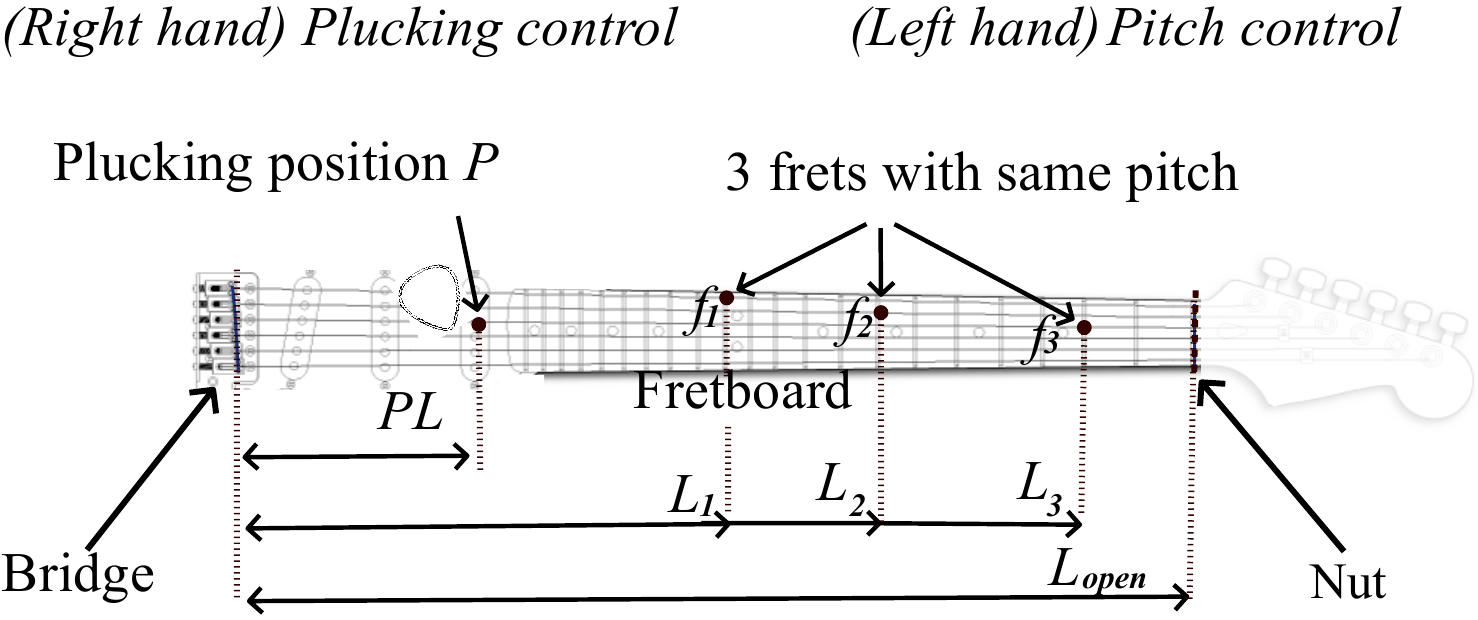
\includegraphics[width=.95\columnwidth]{img/fender_drawing4.png}}
  \caption{The plucking position is controlled by the right hand while the left hand controls pitch using the fretboard. Similar pitch is produced in various positions. Source: Adapted from~\cite{phillips}.
  }\label{fig:guitar_overview}\vspace{-2mm}
\end{figure}
%
The string has an initial deflection $\delta$ at the plucking position $P$, which is at the $P$th fraction of its length $(0<PL<L)$, where $L$ is the length of the vibrating string (see i.e.,~Fig.~\ref{fig:guitar_overview}). Assuming that the string is not ideal and is pinned at locations $l=0$ and $l=L$, its general solution at time $t\geq0$ can be written as a sum of normal modes~\cite{fletcher:physics_of_musical_instruments}
%
\begin{equation}\label{eq:modalSum}
    y(l,t) = \sum_m C_m\sin(\psi_m(\omega_0,B)t+\phi_m)\sin\kappa_ml,
\end{equation}
%
%where we propose to estimate string, fret and plucking position from simulated physical models of the
with fundamental frequency $\omega_0$, inharmonicity coefficient $B$ and amplitude $C_m$, wave number $\kappa_m = m/ 2L$ and phase $\phi_m$ of the $m$th mode. The instantaneous frequency $\psi_m(\omega_0,B)$ follows the piano model proposed in~\cite{fletcher:piano_model} as 
\begin{equation}\label{eq:pianoModel}
  \psi_m(\omega_0,B) = m \omega_0 \sqrt{1+B m^2} \quad [\text{s}^{-1}], 
\end{equation}
that has been proven useful for accurate fundamental frequency estimation~\cite{galembo1994measuring, nillson:multipitch_inharmonic_signals} on stringed instruments and for feature extraction~\cite{michelson2018_aes,abesser2012feature,barbancho:inharmonicity_tablature} with both $\omega_0$ and $B$ as ``black box'' parameters.
Assuming the initial displacement to be triangular with no initial velocity $\frac{\partial y}{\partial t} = 0 \, \forall\, l$, the $m$th amplitude $C_m$ is defined by the Fourier sine series as~\cite{donkin:acoustics,fletcher:principles_of_vibration_and_sound}
\begin{equation}\label{eq:pluck_closed_form}
    C_m = \frac{2\delta}{m^2\pi^2P(1-P)}\sin(m\pi P), \quad [\cdot].
\end{equation}
From~\eqref{eq:pluck_closed_form}, it can be observed that the spectral envelope is sinusoidal along the partials, and dependent only on the plucking position $P$ scaled by $m^{-2}$ for the $m$th mode.

On the guitar we assume that a pickup is measuring the displacement $y(l,t)$ in close proximity to the string at location $l\!=\!\lambda$. At the discrete time instance $n$ the observed signal $x(n)$ is uniformly sampled such that is proportional to $y$, i.e.,
%\begin{equation}
     $x(n)  \vert_{l=\lambda} \propto y(\lambda, t).$
%\end{equation}   
We parametrize $x(n)$ as proposed in~\cite{hjerrild::icassp19}, where $x(n)$ is modeled as an inharmonic sinusoidal part and a noise part, i.e.,  
\begin{equation}\label{eq:sigmod1}
  x(n)\! =  \!\sum\limits_{m=1}^{M}\!\! \alpha_{m} \exp\big({j\psi_m(\omega_0,B) n}\big)+v(n),
\end{equation}
where $\alpha_{m}$ is the complex amplitude of the $m$th partial, $M$ is the number of partials, $v(n)$ is noise and $\psi_m(\omega_0,B)$ is defined in~\eqref{eq:pianoModel}.
%
 At time instance $n$, the observed signal vector $\vecx \in \mathbb{C}^N$ is represented as $\vecx = [x(0) \, x(1) \, \cdots \, x(N-1)]^T$, with $T$ denoting the transpose. 
In matrix notation the observed signal is
\begin{equation}\label{eq:xZa}
  \vecx = \matZ \vecalpha + \vecv,
\end{equation} 
where $\vecalpha\!=\! [\alpha_1 \: \cdots \: \alpha_M]^T$ is a vector containing complex amplitudes, $\vecv\! =\! [v(0) \: v(1) \: v(N-1)]^T$ contains all noise terms and the Vandermonde matrix $\matZ\! \in\! \mathbb{C}^{N\times M}$ contains all inharmonic sinusoids as $\matZ =& \left[ \vecz(\psi_1) \: \vecz(\psi_2) \: \cdots \: \vecz(\psi_M)\right] \matZ \in \mathbb{C}^{N\times M}$, where each column is $\vecz(\psi_m) =& \left[ 1 \: e^{j\psi_m} \: e^{j\psi_m2} \: \cdots \: e^{j\psi_m(N-1)} \right]^{T}$.
We denote the unknown and deterministic parameters that comprises the feature set 
%with $\vectheta$, i.e.
%\begin{equation}\label{eq:theta_parameters}
  $\vectheta = \{\omega_0, B, \vecalpha\}$.
%\end{equation}
The amplitudes $\vecalpha$ are linear, while the fundamental frequency $\omega_0$ and inharmonicity $B$ both are non-linear. 
The amplitude estimates $\vecalphahat$ has been shown to be sufficient for estimating the plucking position $\widehat{P}$ in the fretted string scenario~\cite{hjerrild::icassp19}, while $\{\widehat\omega_0, \widehat B \} $ was sufficient for classification of string and fret in~\cite{barbancho:inharmonicity_tablature,michelson2018_aes}.%
%
%
%%%%%%%%%%%%%%%%%%%%%%%%%%%%%%%%%%%%%%%%%%%%%%%%%%%%%
%%%%%%%%%%%%%%%%%%%% PROPOSED METHOD %%%%%%%%%%%%%%%%
%%%%%%%%%%%%%%%%%%%%%%%%%%%%%%%%%%%%%%%%%%%%%%%%%%%%%
%
\section{Proposed Method}\label{sec:proposed_method}
%To overcome the problem of requiring the user to provide audio recordings and to obtain a class dependent model, we propose a  Monte Carlo simulation of the feature space. 
To overcome the problem of requiring the user to provide audio recordings and to obtain a class dependent model, we propose a physical modeled simulation of the feature space. Instead of requiring audio for the building of a model, as done in~\cite{abesser:automatic_string_detection_ml,barbancho:inharmonicity_tablature,michelson2018_aes,hjerrild::icassp19}, the simulation requires only knowledge of string properties, as explained and derived from physics in the following. The proposed method implicitly increases computational efficiency on two levels; the user is not required to record audio for training, and the model is obtained from one simulation instead of estimating features from several audio recordings. Specifically, the features that we simulate are ${\omega}_0$ and $B$, which have been proven useful for string and fret classification~\cite{barbancho:inharmonicity_tablature, michelson2018_aes,hjerrild::icassp19}. The known string properties are
\begin{itemize}
    \item String length $L \sim \mathcal{N}(\mu_{L}, \,\sigma_{L}^{2} ) $.
    \item String tension $T_0 \sim \mathcal{N}(\mu_{T_0},\,\sigma_{T_0}^{2})$.
    \item Plucking deflection $\delta \sim \mathcal{N}(\mu_{\delta},\,\sigma_{\delta}^{2})$.

    \item Core diameter $ d_c \sim \mathcal{N}(\mu_{d_\text{c}},\,\sigma_{d_\text{c}}^{2})$.
    \item Core density $ \rho_c \sim \mathcal{N}(\mu_{\rho_\text{c}},\,\sigma_{\rho_\text{c}}^{2})$.
    \item Wrapping diameter $ d_w \sim \mathcal{N}(\mu_{d_\text{w}},\,\sigma_{d_\text{w}}^{2})$.
    \item Wrapping density $\rho_w \sim \mathcal{N}(\mu_{\rho_\text{w}},\,\sigma_{\rho_\text{w}}^{2})$.

\end{itemize}
%
We assume that the user knows $\mu_L$ from the guitar-type, and parameters such as $\mu_{T_0}$, $\mu_{d_\text{c}}$, $\mu_{d_\text{w}}$, $\mu_{\rho_\text{c}}$, $\mu_{\rho_\text{w}}$ can be given by string manufacturers and are often printed on the string package. The standard deviations $\sigma$ are specified as 0.5\% of the respective mean value $\mu$ (please see the available code\footnote{\url{https://tinyurl.com/waspaa2019}} ).
%
%
%
%
%
%
% \subsection{Inharmonic pitch definitions for the wrapped string %Introducing the effect of wrapping
% }

% The inharmonicity is highly correlated with the core diameter $d_\text{c}$ and string inharmonicity has been an area of research for more than a century see i.e.,~\cite{rayleigh:sound}. For string designers, it is in general desired to lower the inharmonicity. For low-pitched strings it is not desired to simply increase the core diameter in order to lower the fundamental frequency as inharmonicity will increase by a power of 4 (as can be seen in \eqref{eq:intrinsicInharmonicity}). Therefore the strings are wrapped to add mass to the string to lower the pitch without affecting the inharmonicity by much. (BUT IT DOES A LITTLE: SEE SECTION INCLUDING $T_\text{c}$ AND $T_\text{w}$).

% \noindent The mass per unit length $\mu$ of a wrapped string is defined by:

% \begin{equation}
%     \mu = \frac{\pi}{4}\Big(\rho_\text{c}d_\text{c}^2 + \rho_\text{w}\big[(2d_\text{w}+d_\text{c})^2-d_\text{c}^2\big]\Big), \quad [\text{kg}\cdot\text{m}],
% \end{equation}
% where $d_\text{c}$, $d_\text{w}$ are the core and wrapping diameters and $\rho_\text{c}$, $\rho_\text{w}$ are the densities of the core and wrapping respectively. When the string is single-cored ($d_\text{w} = 0$), and thus not wrapped, the second term becomes zero. Since the tension mainly acts on the core, the string can be considered a single cored string having the same mass per unit length $\mu$, but with the diameter of the core $d_\text{c}$ only. The effective density of this theoretical material is defined as~\cite{firth:string_design} (with $\frac{\pi}{4}$ removed)
% \begin{equation}
%     \rho_{\textup{eff}} = \rho_\text{c} + \rho_\text{w} \big[(1+2\frac{d_\text{w}}{d_\text{c}})^2-1\big], \quad [\text{kg}\cdot\text{m}^{-3}].
% \end{equation}
% This effective density can be used to calculate the fundamental frequency for the string, from the tension and length. The relation between the string length (nut-bridge) $L$, the tension $T_0$ and the fundamental frequency $\omega_0$ is:

% \begin{equation}\label{eq:tension}
%     T_0 = \pi (L\omega_0)^2d_\text{c}^2\rho_{\textup{eff}} = \mu(2L\omega_0)^2, \quad [\text{N}],
% \end{equation}
% from which the equation for fundamental frequency can easily be derived:
% \begin{equation}
%     \omega_0 = \sqrt{\frac{T_0}{\mu}} \frac{1}{2L} \quad [\text{s}^{-1}],
% \end{equation}
% where the mass and length are being considered as constants. 
%
%
%
%
%
The first feature $\omega_0$ for wrapped strings, can be calculated from the mass per unit length $\upsilon$ based on known material densities and diameters \cite{firth1984}
\begin{equation}
    \upsilon = \frac{\pi}{4}\Big(\rho_\text{c}d_\text{c}^2 + \rho_\text{w}\big[(2d_\text{w}+d_\text{c})^2-d_\text{c}^2\big]\Big), \quad [\text{kg}\cdot\text{m}],
\end{equation}
which, together with the given tension $T_0$, can be used to calculate $\omega_0$ as
\begin{equation}\label{eq:omega_0}
    \omega_0 = \sqrt{\frac{T_0}{\mu}} \frac{1}{2L} \quad [\text{s}^{-1}].
\end{equation}
In the following, we extend on the state of the art~\cite{rossing:science_of_string_instruments} by providing a more accurate description of %more precise calculations for different parameters used to calculate 
the inharmonicity coefficient, that will be proven accurate for string and fret classification. %, that is accurate for string and fret classification, as shown. 
After this, we proceed with a description of the feature extraction, based on~\cite{hjerrild::icassp19}.
%
%
\subsection{Simulation of the inharmonicity coefficient}\label{sec:Bsimulation}
The authors of \cite{coltShank} state that string inharmonicity arises from two sources: the intrinsic inharmonicity due to the $\textit{stiffness}$ of the string and inharmonicity due to $\textit{stretching}$ caused by deflection. Using Rossing's quantification of these sources in \cite{rossing:science_of_string_instruments} we propose the inharmonicity coefficient in \eqref{eq:pianoModel} to be an addition of both:
% \begin{align}
%     K = \frac {\pi^3 E d_\text{c}^2}{16 T_0 L^2}, \quad [\text{m}^{-2}],
% \end{align}
\begin{equation}\label{eq:totalInharmonicity}
    B =  \frac {\pi^3 E d_\text{c}^2}{16 T_0 L^2}\left(\frac {d_\text{c}^2}{4}   +  \frac {3\delta^2}{8} \right)  =  \frac{\pi^3 E d_\text{c}^2(2d_\text{c}^2 + 3\delta^2)}{128 T_0 L^2}\quad [\cdot].
\end{equation}
where Young's Modulus $E$ of the string material is defined in \eqref{eq:tensile_stress}.
% The intrinsic inharmonicity and inharmonicity due to plucking with maximum transverse displacement $\delta$ (pluck amplitude) for $P=0.5$, i.e. if the string is plucked at the center, are defined as
% \begin{align}\label{eq:intrinsicInharmonicity}
%     B_\text{i} = \frac {K}{4} d_\text{c}^2\quad \text{and}\quad B_\delta = \frac {3K}{8} \delta^2.
% \end{align}
% and the inharmonicity due to plucking with maximum transverse displacement $\delta$ (pluck amplitude) is  
% \begin{align}\label{eq:displacementInharmonicity}
%     B_\delta = \frac {3K}{8} \delta^2 \quad [\cdot],
% \end{align}
% if $P=0.5$, i.e. if the string is plucked at the center.
%This pitch shift is responsible for the initial twang (\textbf{isn't this twang especially due to higher frequency content at the beginning of the pluck} of the string and dies down rapidly after the pluck. It is assumed
%
% According to~\cite{fletcher:piano_model} the $\textit{intrinsic string inharmonicity}$ $B_i$ is
%
% \begin{equation}
%     B_i = \frac{\pi^2 E A R_g^2}{T L^2}, \quad [\cdot],
% \end{equation}
% where the radius of gyration $R_g^2 = \frac{I}{A} = \frac{\pi}{4}\big(\frac{d_\text{c}}{2}\big)^4 \frac{1}{A}$ assuming a one-dimensional - not planar - radius of gyration
% %
% \begin{equation}\label{eq:intrinsicInharmonicity}
%     B_i =  \frac{\pi^3 E d_\text{c}^4}{64 T L^2} = \frac{\pi^2 E d_\text{c}^2}{64\rho_{\text{eff}} L^4 \omega_0^2}\quad [\cdot].
% \end{equation}
% The total inharmonicity can then be defined as
% \begin{equation}\label{eq:totalInharmonicity}
%     B =  B_\text{i} + B_\delta =  \frac{\pi^3 E d_\text{c}^2(2d_\text{c}^2 + 3\delta^2)}{128 T_0 L^2}\quad [\cdot].
% \end{equation}
% 
%where the inharmonicity coefficient $B$ is a combination of intrinsic inharmonicity and inharmonicity due to plucking:
% 
% 
% 
% as one contribution from string properties and one from the plucking deflection $\delta$, i.e.,
% Rossing  quantifies the physical relations of~\eqref{eq:totalInharmonicity} in~\cite{rossing:science_of_string_instruments}
% with string-core diameter $d_\text{c}$, string-tension $T_0$ and Young's modulus $E$ of the string material defined in \eqref{eq:tensile_stress}.
% 
% \noindent We propose to model the fundamental frequency as 
% % It is clear that we can express the fundamental frequency with the well known equation:
% \begin{equation}
%     \omega_0 = \sqrt{\frac{T_0}{\mu}} \frac{1}{2L_0} \quad [s^{-1}].
% \end{equation}
%
It is expected that $d_\text{c}\ll\delta$, i.e. the plucking deflection is likely to be more than an order of magnitude greater than the string diameter. Hence, the inharmonicity caused by the pluck dominates the intrinsic inharmonicity. However, this is only true immediately after the pluck, as the effect of the former dies down rapidly after the string is excited \cite{rossing:science_of_string_instruments}. %Presumably, this is the reason why the literature on this topic has disregarded the initial displacement in the calculation of inharmonicity. 
As in our application, we solely use the first 40 ms of the plucked string sound, it is of utmost importance to include the effect that the initial displacement has on the total inharmonicity.
%
%\begin{equation}\label{eq:tension}
%    T_0 = \mu(2L\omega_0)^2, \quad [\text{N}],
%\end{equation}
%
\subsubsection{Calculating $\delta$ for an arbitrary plucking-position}
In \cite{rossing:science_of_string_instruments}, for the use of $\delta$ it is assumed that $P=0.5$, i.e. the string is plucked at the center. Realistically, the plucking position will rarely, if not never, be in the middle of the string. We can calculate $\delta$ in \eqref{eq:totalInharmonicity} from the transverse displacement at the $P$th fraction of the string-length $\delta_P$ where $P \neq 0.5$ utilising the change in string length due to plucking. This is calculated using
\begin{equation}\label{eq:changeLengthPluck}
    \Delta L_P = \sqrt{(LP)^2+{\delta_P}^2}+\sqrt{(L(1-P))^2+{\delta_P}^2} - L.
\end{equation}
This length extension can be used to calculate $\delta$ as if the string were plucked in the center. This will also retain the tension present in the string as $T_0$ and $\Delta L$ are proportional according to \eqref{eq:tensile_stress}. Setting $P = 0.5$, we can simplify \eqref{eq:changeLengthPluck} to
%
\begin{equation}\label{eq:changeLengthPluckHalf}
    \Delta L_{0.5} = 2\sqrt{(0.5L)^2 + \delta^2} - L.
\end{equation}
%
Replacing $\Delta L_{0.5}$ with the length extension $\Delta L_P$ calculated in \eqref{eq:changeLengthPluck} and solving \eqref{eq:changeLengthPluckHalf} for $\delta$ yields
\begin{equation}
    \delta = \frac{\sqrt{{\Delta L_P}^2+2L\Delta L_P}}{2},
\end{equation}
which can be used to calculate the inharmonicity due to plucking.

\subsubsection{Calculating $E$ for wrapped strings}%Calculating strain length $\Delta L$ from material properties}
%
When the string is brought to pitch (tuned) it stretches according to its Young's modulus (or elastic modulus) $E$ which is defined as
%
\begin{equation}\label{eq:tensile_stress}
    E = \frac{\text{Tensile stress}}{\text{Strain}}
   %= \frac{T/A_\text{c}}{\Delta L/(L - \Delta L)} 
    = \frac{T_0/A_\text{c}}{\Delta L/(L - \Delta L)} \quad [\text{N}\cdot\text{m}^{-2}], 
\end{equation}
%
where $A_\text{c} = \pi d_\text{c}^2/4$ is the cross-sectional area of the string-core and $\Delta L$ is the amount by which the string is stretched. The variables $E$, $A_\text{c}$ and $L$ are often considered constant and we know that $T_0$ and $\Delta L$ are proportional. Important to note is that we use $L - \Delta L$ to describe the original string length before stretched to $L$. The Young's modulus is a property defined for solid materials. Even though the string core and wrapping could be the same material, the wrapping is not solid! This means that when calculating the total inharmonicity using \eqref{eq:totalInharmonicity} for a wrapped string, the Young's modulus will be incorrect. %The effect of wrapping on the tension is small, though not neglegible. 
More specifically, the total tension $T_0$ will be incorrect as this will now be a combination of
\begin{equation}\label{eq:totalTension}
    T_0 = T_\text{c} + T_\text{w},
\end{equation}
where $T_\text{c}$ is the tension contributed by the core and $T_\text{w}$ the tension contributed by the wrapping. %In the following we present how to correctly calculate Young's modulus $E$ for wrapped strings.
%
%Assuming that we know $A_\text{c}$, $L$ and $T_0$ we need to obtain $\Delta L$ to calculate $E$ in \eqref{eq:tensile_stress}. 
We can assume the wrapping to be a spring as in \cite{kemp:wound_and_unwound_strings} with spring constant~\cite{childs:mechanical_engineering}
%
\begin{equation}\label{eq:k_wrapping}
    k = \frac{Gd_\text{w}^4}{8ND^3}, \quad [\text{N}\cdot\text{m}^{-1}].
\end{equation}
%
Here, $G$ is the shear modulus of the wrapping material, $N = \frac{L - \Delta L}{d_\text{w}}$ is the number of turns in the coil (assuming that for the untensioned string, every coil touches the previous and the next coil) and $D = d_\text{c}+d_\text{w}$ is the mean diameter of the spring~\cite{kemp:wound_and_unwound_strings}.
%
The length extension $\Delta L$ for a spring is
%
\begin{equation}\label{eq:deltaL_wrapping}
    \Delta L = \frac{T_\text{w}}{k} = \frac{8T_\text{w}LD^3}{Gd_\text{w}^5 + 8T_\text{w}D^3} \quad [\text{m}].
\end{equation}
%
For the core of the string we can rewrite~\eqref{eq:tensile_stress}, i.e.,
%
\begin{equation}\label{eq:deltaL}
    \Delta L= \frac{LT_\text{c}}{A_\text{c}E + T_\text{c}}, \quad  [\text{m}], 
\end{equation}
%
and as the core and wrapping are part of the same string, they undergo the same length-extension $\Delta L$, meaning that we can set \eqref{eq:deltaL_wrapping} and \eqref{eq:deltaL} equal to each other and -- recalling~\eqref{eq:totalTension} -- we can solve for $T_\text{w}$ and $T_\text{c}$
% %
% \begin{equation}\label{eq:deltaLtw} \frac{LT_\text{c}}{A_\text{c}E + T_\text{c}} = \frac{8D^3LT_\text{w}}{Gd_\text{w}^5 + 8D^3T_\text{w}}.
% \end{equation}
%
% As we know the desired tension $T_0$ through~\eqref{eq:tension} and r
% Recalling, we can calculate the effect of the core and wrapping tensions:
%
\begin{equation}
    T_\text{w} = \frac{GT_0d_\text{w}^5}{Gd_\text{w}^5 + 8A_\text{c}D^3E}, \ \ T_\text{c} = \frac{8A_\text{c}D^3ET_0}{Gd_\text{w}^5+8A_\text{c}D^3E}\quad [\text{N}].
\end{equation}
%
% An alternative way to calculate the contributions of $T_\text{c}$ and $T_\text{w}$ on the total tension is to compute their ratio $T_{c/w}$. This simplifies the above definitions to
% %
% \begin{equation}
%     T_{c/w} = \frac{T_\text{c}}{T_\text{w}} = \frac{8A_\text{c}D^3E}{Gd_\text{w}^5},  \quad [\cdot],
% \end{equation}
% %
% and can be used to calculate $T_\text{c}$ and $T_\text{w}$ by
% %
% \begin{equation}\label{eq:Tc_derived}
%     %T_\text{c} (\frac{1}{\tau_{c/w}}+1) = T_0, \qquad T_\text{w} (\tau_{c/w} + 1) = T_0,  \\
%     T_\text{c} = \frac{T_0}{\frac{1}{T_{c/w}}+1}, \quad T_\text{w} = \frac{T_0}{T_{c/w}+1}\quad [\text{N}].
% \end{equation}
%
Finally, inserting $T_\text{w}$ into \eqref{eq:deltaL_wrapping} or $T_\text{c}$ into \eqref{eq:deltaL}, gives the length extension based on the string-material properties of both core and wrapping, which can then be used in \eqref{eq:tensile_stress} to calculate the correct Young's modulus $E$.

This concludes the derivations used for the proposed method of simulating the feature set $\{\omega_0, B\}$. In the following we explain how to estimate these from the observed signal $\vecx$.

\subsection{Estimation of String, Fret and Plucking Position}
\subsubsection{Inharmonic Partial Estimation}
The feature set $\boldsymbol{\theta}$ is extracted by maximizing the likelihood function %probability of the observed data $\vecx$ given the parameters:
\begin{equation}
    \thetahat = \argmax{\vectheta}{\Like(\vectheta | \vecx)} = \argmax{\vectheta}{p(\vecx ; \vectheta)}.
\end{equation}
The observed signal distribution is modeled in circular complex white Gaussian noise, and as derived in~\cite{hjerrild::icassp19} a computationally efficient approach can be found as
\begin{equation} \label{eq:ANLS}
    \{\widehat\omega_0, \widehat B \} = \argmax{\omega_0,B}{\vecx^H \matZ \matZ^H \vecx} = \argmax{\omega_0,B}{ \norm{\matZ^H\vecx}_2^2},
\end{equation}
which can be implemented using just one FFT per segment, i.e.,
\begin{equation}
    	\{\widehat\omega_0,\widehat B  \} = \underset{\{\omega_0, B  \}}{\operatorname{argmax}}\; \sum_{m=1}^{M} |X(\psi_m(\omega_0,B))|^2, 
\end{equation}
with $X$ being the FFT of $\vecx$. To ease computational complexity an initial fundamental frequency estimate is obtained with $B=0$, and then a two dimensional search grid is defined for estimating  $\{\widehat\omega_0, \widehat B \}$. % An optimal grid can be selected using~\cite{jkn:grid_size}. 
 Finally, the inharmonic partials are found as least squares estimates, i.e.,
\begin{equation}\label{eq:alphahat}
  \vecalphahat = (\Z^H\Z)^{-1}\Z^H\vecx.
\end{equation}
\subsubsection{Classification of String and Fret}\label{sec:classifier}
Having found the fundamental frequency and the inharmonicity parameters $\boldsymbol{\phi} = [\widehat{\omega}_0, \widehat{B} ]^T$ from the observed signal snapshot $\vecx$, the next step is classification of the observed signal as being produced from a string and fret combination. 
We have a set of $K$ mutually exclusive classes $\boldsymbol{\Gamma}=\{\gamma_1,\dots,\gamma_K\}$ representing all possible string and fret combinations. The MAP-optimal classifier with decision function $\hat{\gamma}(\cdot): \mathbb{R}^I \rightarrow \boldsymbol{\Gamma}  $ is 
\begin{align}
    \hat\gamma_{{MAP}}(\boldsymbol{\phi}) &= \underset{\gamma\in\Gamma}{\operatorname{argmax}}\;{p(\gamma|\boldsymbol{\phi})} = \underset{\gamma\in\Gamma}{\operatorname{argmax}}\;{p(\boldsymbol{\phi}|\gamma)P(\gamma)}.
\end{align}
We model $\boldsymbol{\phi}$ as coming from a normal object with class $\gamma_k$, then the $k$th conditional probability density is   
%\begin{equation}
    $p(\gamma_k\lvert\boldsymbol{\phi}) =
    \mathcal{N}(\boldsymbol{\mu}_k,\,\boldsymbol{\Lambda}_k)$ %\, ,
    %{{(2\pi)^{-1}\det{\boldsymbol{\Lambda}_k)^{\frac{-1}{2}}}}}\, \exp\bigg(\frac{-(\boldsymbol{\phi}-\boldsymbol{\mu}_k)^T\boldsymbol{\Lambda}_k^{-1} (\boldsymbol{\phi}-\boldsymbol{\mu}_k) }{2} \bigg),
%\end{equation}
where the expectation vector $\boldsymbol{\mu}_k$ and covariance matrix $\boldsymbol{ \Lambda }_k$ is computed from a Monte Carlo simulation with~\eqref{eq:omega_0} and~\eqref{eq:totalInharmonicity}, where we assume the physical properties of the strings are normally distributed random variables. The covariance matrices are here modeled as being class dependent as compared to the state of the art~\cite{hjerrild::icassp19}, which we shall see, makes way for improved accuracy in the string and fret classification. %Furthermore, it does not require the user to record any audio for training the model, which lowers the computational cost and improves usability and the model can easily be adapted to another set of strings.
%
Neglecting terms that do not depend on the class index $k$ yields the following, classification scheme $\hat{\gamma}(\boldsymbol{\phi})={\gamma}_i$, with
%
\begin{equation}\label{eq:classifier}
%  \hat{\gamma}(\boldsymbol{\phi})={\gamma}_i \quad{\textup{with}}\quad 
  i\!=\!\underset{k=1,\dots,K}{\operatorname{argmax\!\!\!\!\!}}\;
\bigg\{\!\!\! -\!\ln \lvert \boldsymbol{\Lambda}_k\! \rvert\! +\! 2 \!\ln P(\!\gamma_k\!) \!-\! (\boldsymbol{\phi}-\boldsymbol{\mu}_k)^T \boldsymbol{\Lambda}_k^{\!-1} (\boldsymbol{\phi}-\boldsymbol{\mu}_k)    %\frac{\left\lVert{\boldsymbol{\phi}-\boldsymbol{\mu}_k}\right\rVert^2}{\sigma^2} 
\!\!\bigg\}.
\end{equation}
%
%As can be seen, this classifier is the minimizer of the Euclidean distance between the observation and its expectation, with a correction factor of $2\sigma^2 P(\gamma_k)$. 
The prior $P(\gamma_k)$ can be specified from the number of simulation samples from class $\gamma_k$ or be assumed uniform, in which case it reduces to a maximum likelihood classifier, see i.e.,~\cite{mspr}.
%
\vspace{-.8mm}
\subsubsection{Plucking Position Estimation} % (fold)
\label{sec:proposed_estimation_of_pluck_amplitude}
\vspace{-.6mm}
As demonstrated in~\cite{hjerrild::icassp19}, once the partial amplitudes has been estimated using~\eqref{eq:alphahat}, the plucking position $\widehat{P}$ can be found. As proposed in~\cite{hjerrild::icassp19} we minimize the log spectral (LS) distance between the observation $\vecalphahat$ and the model $\mathbf{C}$ to find $\widehat{P}$, i.e., 
\begin{equation}
    \widehat{P} = \argmin{P}{\big(d_{\textup{LS}}(\vecalphahat,\mathbf{C}(P))\big)},
\end{equation}
where $\mathbf{C}(P) = [C_1(P),C_2(P),\dots,C_M(P)]^T$ is obtained from the model in~\eqref{eq:pluck_closed_form} and the log spectral distortion is defined as
\begin{equation}
    d_{\textup{LS}}(\vecalphahat,\mathbf{C}(P)) = \sqrt{ \frac{1}{M} \sum_m 10\log_{10} \frac{\lvert\widehat{\alpha}_m\rvert^2}{\lvert C_m(P)\rvert^2} }.
\end{equation} 
%We remark that the model $\mathbf{C}$ can be more physically meaningful by combining it with a model of the pickup location, such as e.g.,,~\cite{DBLP:conf/icassp/MohamadDH17}.\vspace{-2mm}
%
%
%
%
% ---- EVALUATION 
%
%
\section{Evaluation} % (fold)
\label{sec:experiments}
\input evaluation.tex
%
%
%
% ----- CONCLUSION
%
%
%
\section{Conclusion}
In this paper a method for analyzing guitar performances is proposed. This method extracts the activated string and fret as well as the plucking position, and it is purely based on a physical model of string excitation and vibration, hence it does not require any training data which makes it fast and effective. Since it operates on a 40 ms segment-by-segment basis it is suitable for real-time estimation...
  %Maybe something along the lines of:\\
%Now that we have included plucking position to calculate the initial displacement $\delta$ we might be able to also estimate this. 
%
% -------------------------------------------------------------------------
% Either list references using the bibliography style file IEEEtran.bst

\pagebreak
\bibliographystyle{IEEEtran}
\bibliography{myabbr,refs17,refs}
%
% or list them by yourself
% \begin{thebibliography}{9}
% 
% \bibitem{waspaa17web}
%   \url{http://www.waspaa.com}.
%
% \bibitem{IEEEPDFSpec}
%   {PDF} specification for {IEEE} {X}plore$^{\textregistered}$,
%   \url{http://www.ieee.org/portal/cms_docs/pubs/confstandards/pdfs/IEEE-PDF-SpecV401.pdf}.
%
% \bibitem{PDFOpenSourceTools}
%   Creating high resolution {PDF} files for book production with 
%   open source tools, 
%   \url{http://www.grassbook.org/neteler/highres_pdf.html}.
%
% \bibitem{eWilliams1999}
% E. Williams, \emph{Fourier Acoustics: Sound Radiation and Nearfield Acoustic
%   Holography}. London, UK: Academic Press, 1999.
% 
% \bibitem{ieeecopyright}
%   \url{http://www.ieee.org/web/publications/rights/copyrightmain.html}.
%
% \bibitem{cJones2003}
% C. Jones, A. Smith, and E. Roberts, ``A sample paper in conference
%   proceedings,'' in \emph{Proc. IEEE ICASSP}, vol. II, 2003, pp. 803--806.
% 
% \bibitem{aSmith2000}
% A. Smith, C. Jones, and E. Roberts, ``A sample paper in journals,'' 
%   \emph{IEEE Trans. Signal Process.}, vol. 62, pp. 291--294, Jan. 2000.
% 
% \end{thebibliography}


\end{sloppy}
\end{document}
